\documentclass[11pt,a4paper]{report}
\usepackage[textwidth=37em,vmargin=30mm]{geometry}
\usepackage{calc,xunicode,amsmath,amssymb,paralist,enumitem,tabu,booktabs,datetime2,xeCJK,xeCJKfntef,listings}
\usepackage{tocloft,fancyhdr,tcolorbox,xcolor,graphicx,eso-pic,xltxtra,xelatexemoji}

\newcommand{\envyear}[0]{2025}
\newcommand{\envdatestr}[0]{2025-02-24}
\newcommand{\envfinaldir}[0]{webdb/2025/20250224/final}

\usepackage[hidelinks]{hyperref}
\hypersetup{
    colorlinks=false,
    pdfpagemode=FullScreen,
    pdftitle={Web Digest - \envdatestr}
}

\setlength{\cftbeforechapskip}{10pt}
\renewcommand{\cftchapfont}{\rmfamily\bfseries\large\raggedright}
\setlength{\cftbeforesecskip}{2pt}
\renewcommand{\cftsecfont}{\sffamily\small\raggedright}

\setdefaultleftmargin{2em}{2em}{1em}{1em}{1em}{1em}

\usepackage{xeCJK,xeCJKfntef}
\xeCJKsetup{PunctStyle=plain,RubberPunctSkip=false,CJKglue=\strut\hskip 0pt plus 0.1em minus 0.05em,CJKecglue=\strut\hskip 0.22em plus 0.2em}
\XeTeXlinebreaklocale "zh"
\XeTeXlinebreakskip = 0pt


\setmainfont{Brygada 1918}
\setromanfont{Brygada 1918}
\setsansfont{IBM Plex Sans}
\setmonofont{JetBrains Mono NL}
\setCJKmainfont{Noto Serif CJK SC}
\setCJKromanfont{Noto Serif CJK SC}
\setCJKsansfont{Noto Sans CJK SC}
\setCJKmonofont{Noto Sans CJK SC}

\setlength{\parindent}{0pt}
\setlength{\parskip}{8pt}
\linespread{1.15}

\lstset{
	basicstyle=\ttfamily\footnotesize,
	numbersep=5pt,
	backgroundcolor=\color{black!5},
	showspaces=false,
	showstringspaces=false,
	showtabs=false,
	tabsize=2,
	captionpos=b,
	breaklines=true,
	breakatwhitespace=true,
	breakautoindent=true,
	linewidth=\textwidth
}






\newcommand{\coverpic}[2]{
    % argv: itemurl, authorname
    Cover photo by #2~~(\href{#1}{#1})
}
\newcommand{\makeheader}[0]{
    \begin{titlepage}
        % \newgeometry{hmargin=15mm,tmargin=21mm,bmargin=12mm}
        \begin{center}
            
            \rmfamily\scshape
            \fontspec{BaskervilleF}
            \fontspec{Old Standard}
            \fontsize{59pt}{70pt}\selectfont
            WEB\hfill DIGEST
            
            \vfill
            % \vskip 30pt
            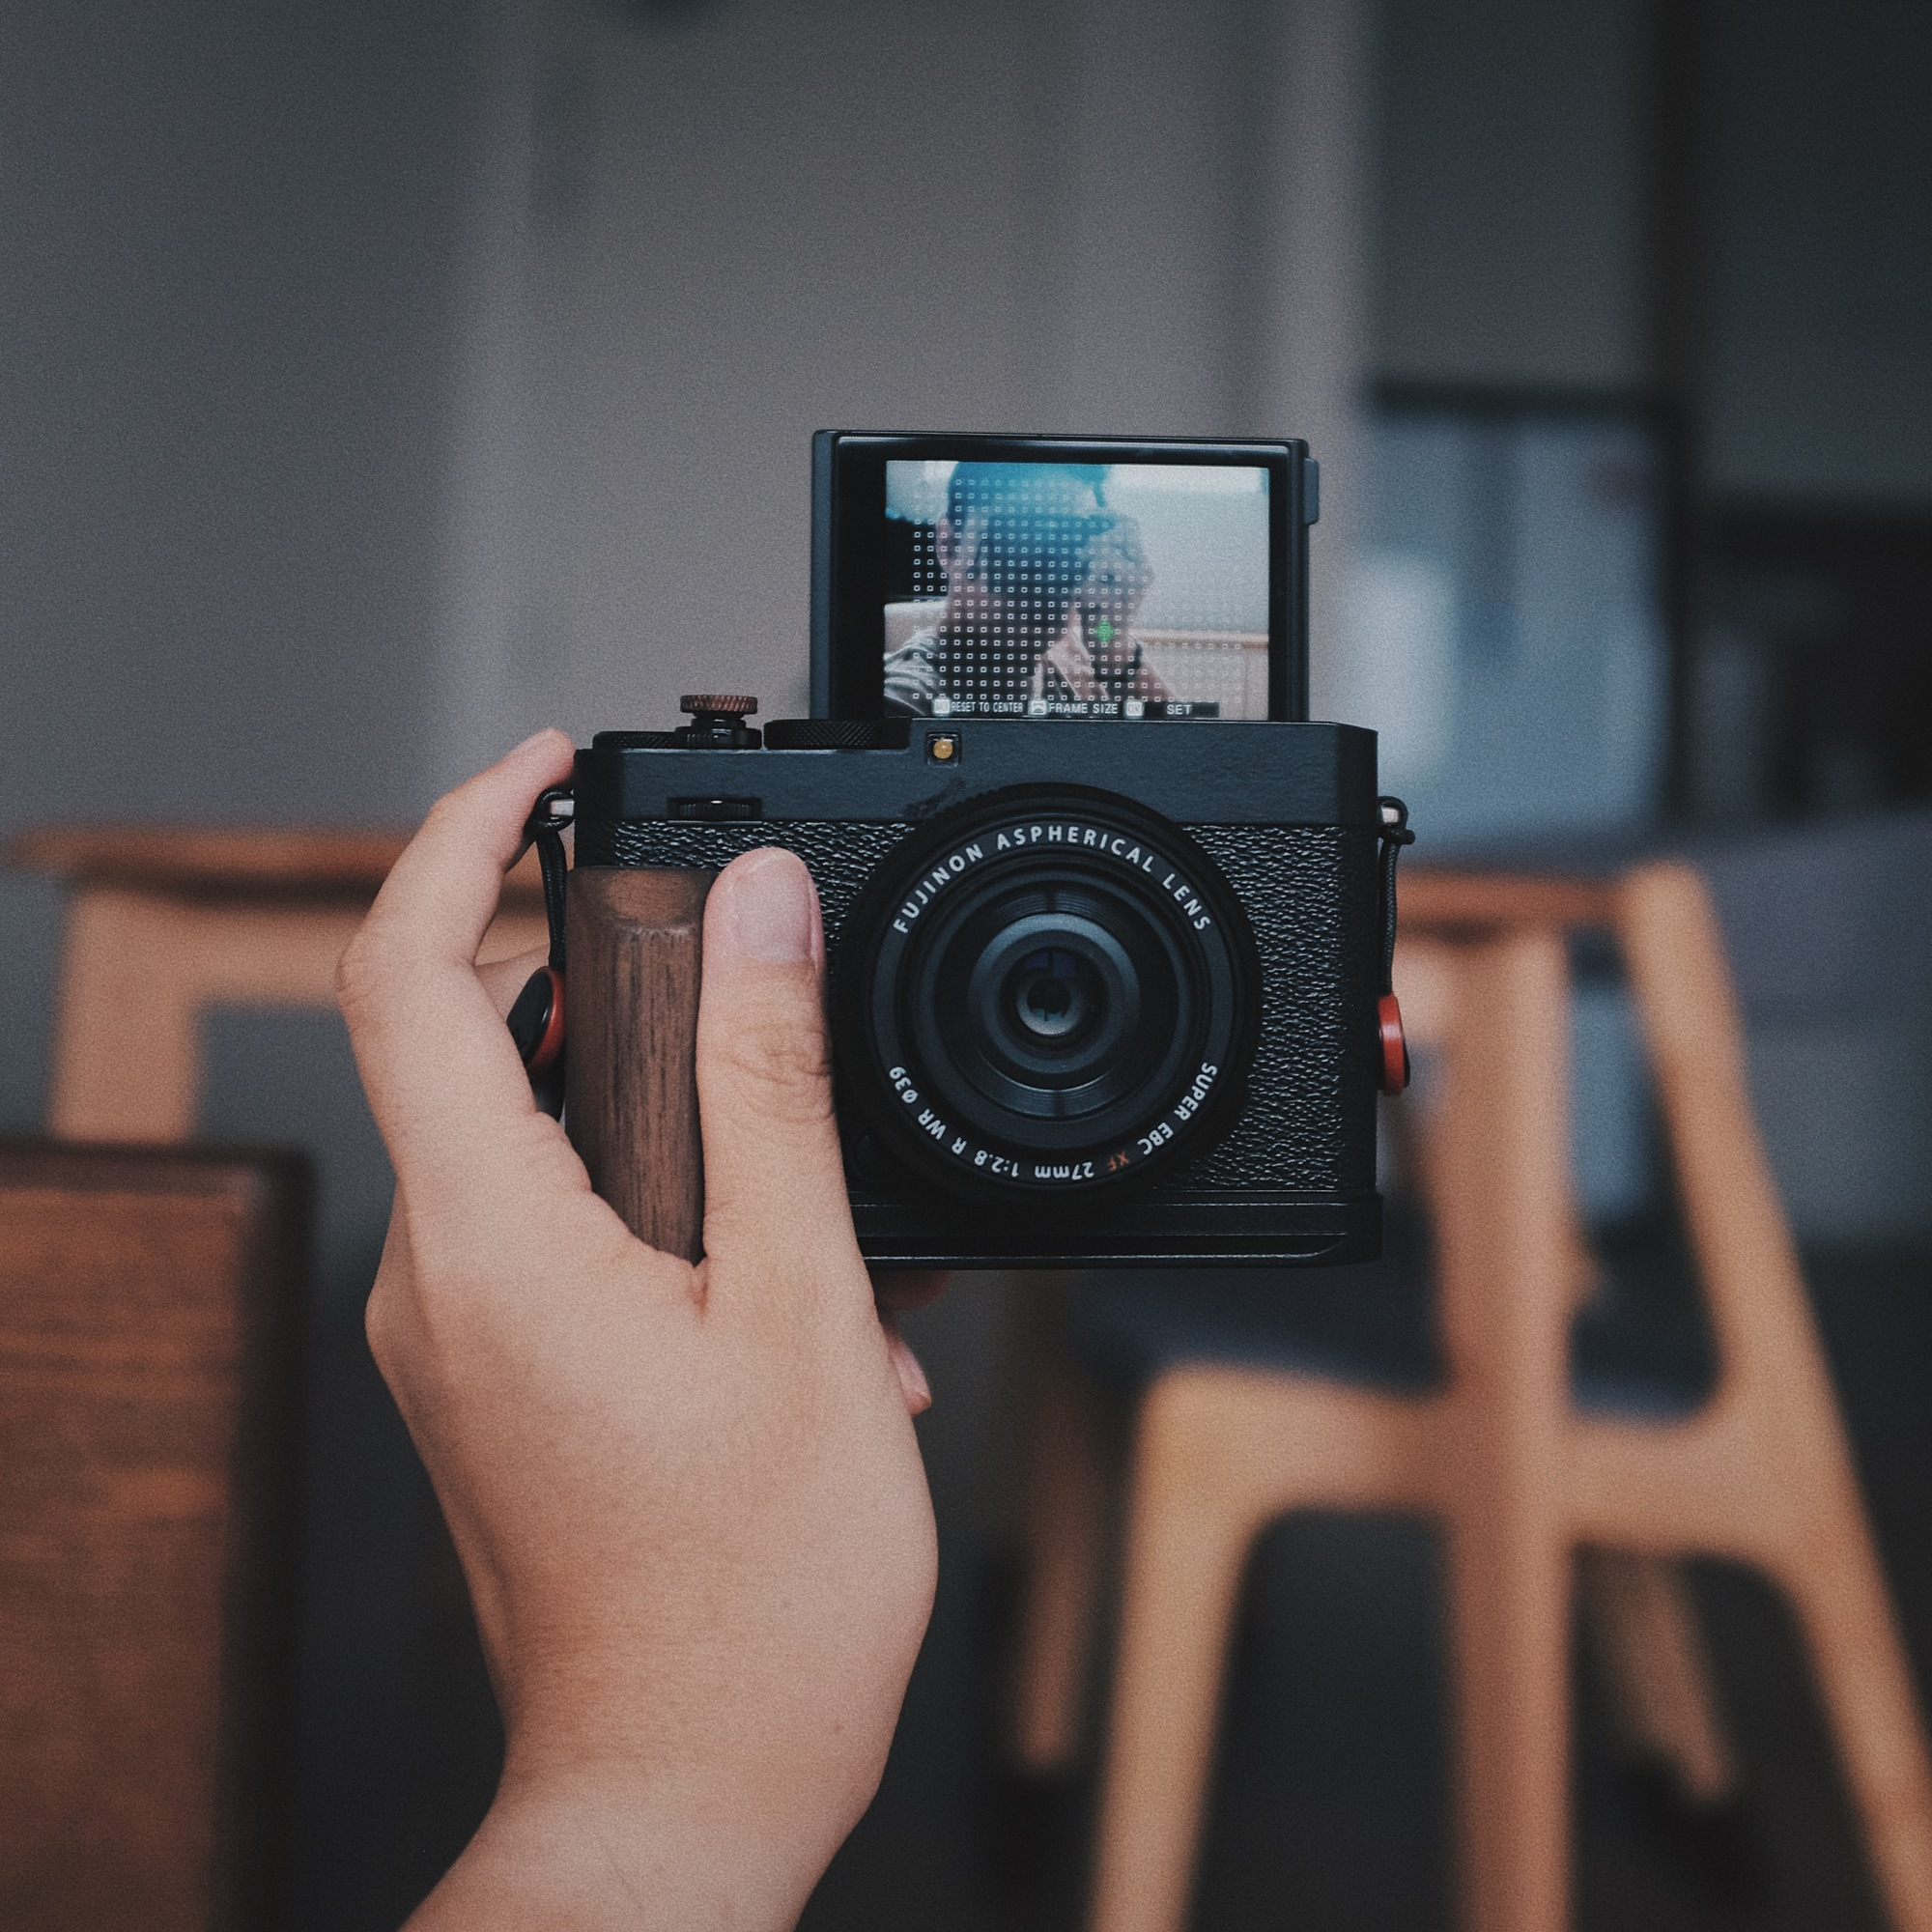
\includegraphics[width=\linewidth]{\envfinaldir/coverpic-prod.jpg}\par
            % \vskip 30pt
            \vfill

            \normalsize\rmfamily\scshape
            \copyright{} The Web Digest Project \hfill\large \envdatestr
        \end{center}
    \end{titlepage}
    % \restoregeometry
}
\newcommand{\simplehref}[1]{%
    \textcolor{blue!80!green}{\href{#1}{#1}}%
}
\renewcommand{\contentsname}{\center\Huge\sffamily\bfseries Contents\par\vskip 20pt}
\newcounter{ipartcounter}
\setcounter{ipartcounter}{0}
\newcommand{\ipart}[1]{
    % \vskip 20pt
    \clearpage
    \stepcounter{ipartcounter}
    \phantomsection
    \addcontentsline{toc}{chapter}{#1}
    % \begin{center}
    %     \Huge
    %     \sffamily\bfseries
    %     #1
    % \end{center}
    % \vskip 20pt plus 7pt
}
\newcounter{ichaptercounter}
\setcounter{ichaptercounter}{0}
\newcommand{\ichapter}[1]{
    % \vskip 20pt
    \clearpage
    \stepcounter{ichaptercounter}
    \phantomsection
    \addcontentsline{toc}{section}{\numberline{\arabic{ichaptercounter}}#1}
    \begin{center}
        \Huge
        \sffamily\bfseries
        #1
    \end{center}
    \vskip 20pt plus 7pt
}
\newcommand{\entrytitlefont}[1]{\subsection*{\raggedright\Large\sffamily\bfseries#1}}
\newcommand{\entryitemGeneric}[2]{
    % argv: title, url
    \parbox{\linewidth}{
        \entrytitlefont{#1}\par\vskip 5pt
        \footnotesize\ttfamily\mdseries
        \simplehref{#2}
    }\vskip 11pt plus 11pt minus 1pt
}
\newcommand{\entryitemGithub}[3]{
    % argv: title, url, desc
    \parbox{\linewidth}{
        \entrytitlefont{#1}\par\vskip 5pt
        \footnotesize\ttfamily\mdseries
        \simplehref{#2}\par\vskip 5pt
        \small\rmfamily\mdseries#3
    }\vskip 11pt plus 11pt minus 1pt
}
\newcommand{\entryitemAp}[3]{
    % argv: title, url, desc
    \parbox{\linewidth}{
        \entrytitlefont{#1}\par\vskip 5pt
        \footnotesize\ttfamily\mdseries
        \simplehref{#2}\par\vskip 5pt
        \small\rmfamily\mdseries#3
    }\vskip 11pt plus 11pt minus 1pt
}
\newcommand{\entryitemHackernews}[3]{
    % argv: title, hnurl, rawurl
    % \parbox{\linewidth}{
    %     \entrytitlefont{#1}\par\vskip 5pt
    %     \footnotesize\ttfamily\mdseries
    %     \simplehref{#3}\par
    %     \textcolor{black!50}{\href{#2}{#2}}
    % }\vskip 11pt plus 11pt minus 1pt
    \begin{minipage}{\linewidth}
            \entrytitlefont{#1}\par\vskip 5pt
            \footnotesize\ttfamily\mdseries
            \simplehref{#3}\par
            \textcolor{black!50}{\href{#2}{#2}}
    \end{minipage}\par\vskip 11pt plus 11pt minus 1pt
}







\begin{document}

\makeheader

\tableofcontents\clearpage




\ipart{Developers}
\ichapter{Hacker News}
\entryitemTwoLinks{Show HN: Jq-Like Tool for Markdown}{https://news.ycombinator.com/item?id=43152704}{https://github.com/yshavit/mdq}

\entryitemTwoLinks{Lobsters blocking UK users because of the Online Safety Act}{https://news.ycombinator.com/item?id=43152178}{https://lobste.rs/s/ukosa1/uk\_users\_lobsters\_needs\_your\_help\_with}

\entryitemTwoLinks{In memoriam}{https://news.ycombinator.com/item?id=43152154}{https://onlinesafetyact.co.uk/in\_memoriam/}

\entryitemTwoLinks{Grok 3 claims its system prompt includes censorship about Musk/Trump}{https://news.ycombinator.com/item?id=43151580}{https://old.reddit.com/r/OpenAI/comments/1iw8eok/elon\_musk\_is\_trying\_to\_censor\_grok\_3\_which\_the/}

\entryitemTwoLinks{Decades of Research Misconduct Stalled an Alzheimer's Cure}{https://news.ycombinator.com/item?id=43151320}{https://www.sciencefriday.com/articles/doctored-book-excerpt/}

\entryitemTwoLinks{WhiteSur: macOS-like theme for GTK desktops}{https://news.ycombinator.com/item?id=43151294}{https://github.com/vinceliuice/WhiteSur-gtk-theme}

\entryitemTwoLinks{Ultima VII: Revisited}{https://news.ycombinator.com/item?id=43150217}{https://www.u7revisited.com/}

\entryitemTwoLinks{It is no longer safe to move our governments and societies to US clouds}{https://news.ycombinator.com/item?id=43150085}{https://berthub.eu/articles/posts/you-can-no-longer-base-your-government-and-society-on-us-clouds/}

\entryitemTwoLinks{Making any integer with four 2s}{https://news.ycombinator.com/item?id=43149883}{https://eli.thegreenplace.net/2025/making-any-integer-with-four-2s/}

\entryitemTwoLinks{'Everybody is looking at their phones,' says man freed after 30 years in prison}{https://news.ycombinator.com/item?id=43149736}{https://news.sky.com/story/everybody-is-looking-at-their-phones-says-man-freed-after-30-years-in-prison-13315407}

\entryitemTwoLinks{Pee If You Want to Go Deeper (2021)}{https://news.ycombinator.com/item?id=43149648}{https://peeifyouwanttogofaster.com/2021/05/24/pee-if-you-want-to-go-deeper/}

\entryitemTwoLinks{Vietnamese Graphic Design}{https://news.ycombinator.com/item?id=43149266}{https://vietgd.com/}

\entryitemTwoLinks{BYD has already produced its first solid-state cells}{https://news.ycombinator.com/item?id=43148697}{https://www.electrive.com/2025/02/17/byd-has-already-produced-its-first-solid-state-cells/}

\entryitemTwoLinks{War Rooms vs. Deep Investigations}{https://news.ycombinator.com/item?id=43148683}{https://rachelbythebay.com/w/2025/02/22/war/}

\entryitemTwoLinks{But good sir, what is electricity?}{https://news.ycombinator.com/item?id=43148438}{https://lcamtuf.substack.com/p/but-good-sir-what-is-electricity}

\entryitemTwoLinks{Half-Life}{https://news.ycombinator.com/item?id=43147698}{https://www.filfre.net/2024/12/half-life/}

\entryitemTwoLinks{No One Lives Forever (NOLF) Revival Edition}{https://news.ycombinator.com/item?id=43146581}{http://nolfrevival.tk/}

\entryitemTwoLinks{Studies correlating IQ to genius are mostly bad science}{https://news.ycombinator.com/item?id=43146274}{https://www.theseedsofscience.pub/p/your-iq-isnt-160-no-ones-is}

\entryitemTwoLinks{Thailand to Cut Power to Myanmar Scam Hubs}{https://news.ycombinator.com/item?id=43146155}{https://bangkoklocal.info/2025/02/05/thailand-to-cut-power-to-myanmar-scam-hubs/}

\entryitemTwoLinks{U. of Pittsburgh pauses Ph.D. admissions amid research funding uncertainty}{https://news.ycombinator.com/item?id=43145483}{https://www.wesa.fm/health-science-tech/2025-02-21/university-pittsburgh-phd-pause-research-funding-uncertainty}\ichapter{Phoronix}
\entryitemGeneric{\hskip 0pt{}Linux 6.14-rc4 Released: The Right Kind Of "Boring"}{https://www.phoronix.com/news/Linux-6.14-rc4}

\entryitemGeneric{\hskip 0pt{}GNU Emacs 30.1 Released With Android Support, Emacs Lisp Native Compiler By Default}{https://www.phoronix.com/news/GNU-Emacs-30.1-Released}

\entryitemGeneric{\hskip 0pt{}Valve Snuck The Lenovo Legion Go S Controller Support Into The Linux Kernel}{https://www.phoronix.com/news/Legion-Go-S-Controller-Linux}

\entryitemGeneric{\hskip 0pt{}AMD Preparing New GPU Support For Their Kernel Graphics Driver In Linux 6.15}{https://www.phoronix.com/news/AMDGPU-Linux-6.15}

\entryitemGeneric{\hskip 0pt{}OneXPlayer Linux Driver Catching Up To The Windows Monitoring Driver}{https://www.phoronix.com/news/OneXPlayer-Linux-Driver-2025}

\entryitemGeneric{\hskip 0pt{}SVT-AV1 3.0 Released With Faster CPU-Based AV1 Encoding}{https://www.phoronix.com/news/SVT-AV1-3.0-Released}

\entryitemGeneric{\hskip 0pt{}Mesa's Venus Now Exposes Vulkan 1.4 Support}{https://www.phoronix.com/news/Mesa-Venus-Vulkan-1.4}

\entryitemGeneric{\hskip 0pt{}Wine Staging 10.2 Adds Support For AF\_UNIX Sockets}{https://www.phoronix.com/news/Wine-Staging-10.2}

\entryitemGeneric{\hskip 0pt{}Microsoft Makes More Of Their DirectX Compiler Code Open-Source}{https://www.phoronix.com/news/DirectXShaderCompiler-2025}\ichapter{Dribbble}
\entryitemGeneric{\hskip 0pt{}Business illustration set}{https://dribbble.com/shots/25661493-Business-illustration-set}

\entryitemGeneric{\hskip 0pt{}Form Golf ID}{https://dribbble.com/shots/25660910-Form-Golf-ID}

\entryitemGeneric{\hskip 0pt{}Shooting Ladybug - Make a wish! Nagare Mushi}{https://dribbble.com/shots/25659882-Shooting-Ladybug-Make-a-wish-Nagare-Mushi}

\entryitemGeneric{\hskip 0pt{}Futuristic aesthetics landing page with Web3 gaming innovation}{https://dribbble.com/shots/25658247-Futuristic-aesthetics-landing-page-with-Web3-gaming-innovation}

\entryitemGeneric{\hskip 0pt{}Puzzle Fintech Website Design [Case Study]}{https://dribbble.com/shots/25478108-Puzzle-Fintech-Website-Design-Case-Study}

\entryitemGeneric{\hskip 0pt{}Sugar Glider Logo}{https://dribbble.com/shots/25653559-Sugar-Glider-Logo}

\entryitemGeneric{\hskip 0pt{}Pendleton Whisky}{https://dribbble.com/shots/25650439-Pendleton-Whisky}

\entryitemGeneric{\hskip 0pt{}Form Golf Wordmark}{https://dribbble.com/shots/25655786-Form-Golf-Wordmark}

\entryitemGeneric{\hskip 0pt{}Logo Design for Ai Assistant Part One}{https://dribbble.com/shots/25652926-Logo-Design-for-Ai-Assistant-Part-One}

\entryitemGeneric{\hskip 0pt{}Gee AI}{https://dribbble.com/shots/25655258-Gee-AI}

\entryitemGeneric{\hskip 0pt{}Living room}{https://dribbble.com/shots/25652845-Living-room}

\entryitemGeneric{\hskip 0pt{}Cimet Software Business Cards}{https://dribbble.com/shots/25648529-Cimet-Software-Business-Cards}

\entryitemGeneric{\hskip 0pt{}Enso Homes Logomark}{https://dribbble.com/shots/25632132-Enso-Homes-Logomark}

\entryitemGeneric{\hskip 0pt{}Fintech UI Design}{https://dribbble.com/shots/25647596-Fintech-UI-Design}

\entryitemGeneric{\hskip 0pt{}Flextro - Logo Design Update}{https://dribbble.com/shots/25648485-Flextro-Logo-Design-Update}

\entryitemGeneric{\hskip 0pt{}Reign - Logotype Design}{https://dribbble.com/shots/25639247-Reign-Logotype-Design}

\entryitemGeneric{\hskip 0pt{}E + Chart Logo Animation}{https://dribbble.com/shots/25640702-E-Chart-Logo-Animation}

\entryitemGeneric{\hskip 0pt{}Pigeon}{https://dribbble.com/shots/25641861-Pigeon}

\entryitemGeneric{\hskip 0pt{}Minimalist S Logo // For Sale}{https://dribbble.com/shots/25641404-Minimalist-S-Logo-For-Sale}

\entryitemGeneric{\hskip 0pt{}Mobile App for a Wellbeing Product ✦ Routine Hero}{https://dribbble.com/shots/25640481-Mobile-App-for-a-Wellbeing-Product-Routine-Hero}

\entryitemGeneric{\hskip 0pt{}Recruitment Dashboard}{https://dribbble.com/shots/25605862-Recruitment-Dashboard}

\entryitemGeneric{\hskip 0pt{}Smart Home Hub}{https://dribbble.com/shots/25637672-Smart-Home-Hub}

\entryitemGeneric{\hskip 0pt{}Lume responsive}{https://dribbble.com/shots/25638482-Lume-responsive}

\entryitemGeneric{\hskip 0pt{}Form Golf Monogram}{https://dribbble.com/shots/25643873-Form-Golf-Monogram}


\ipart{Developers~~~~(zh-Hans)}
\ichapter{Solidot}
\entryitemGeneric{\hskip 0pt{}WinRAR 7.10 允许用户移除可能泄露隐私的元数据}{https://www.solidot.org/story?sid=80622}

\entryitemGeneric{\hskip 0pt{}惠普终止了强制性的电话支持 15 分钟等候时间}{https://www.solidot.org/story?sid=80621}

\entryitemGeneric{\hskip 0pt{}Bybit 被盗走价值 15 亿美元的加密货币}{https://www.solidot.org/story?sid=80620}

\entryitemGeneric{\hskip 0pt{}苹果停止为英国 iCloud 用户提供端对端加密}{https://www.solidot.org/story?sid=80619}

\entryitemGeneric{\hskip 0pt{}Linus Torvalds 回应内核合并 Rust 代码争议}{https://www.solidot.org/story?sid=80618}

\entryitemGeneric{\hskip 0pt{}当你的姓氏是 Null}{https://www.solidot.org/story?sid=80617}

\entryitemGeneric{\hskip 0pt{}250 万年前的超新星爆发可能影响了地球病毒的演化}{https://www.solidot.org/story?sid=80616}

\entryitemGeneric{\hskip 0pt{}Meta 称它下载了盗版电子书库但没有做种不违法}{https://www.solidot.org/story?sid=80615}

\entryitemGeneric{\hskip 0pt{}惠普有意为电话支持加入 15 分钟的等待时间}{https://www.solidot.org/story?sid=80614}

\entryitemGeneric{\hskip 0pt{}ChatGPT 周活跃用户突破 4 亿}{https://www.solidot.org/story?sid=80613}

\entryitemGeneric{\hskip 0pt{}英国研究发现热饮与食管癌相关}{https://www.solidot.org/story?sid=80612}

\entryitemGeneric{\hskip 0pt{}日本将引入数字教科书}{https://www.solidot.org/story?sid=80611}

\entryitemGeneric{\hskip 0pt{}研究发现山东济宁第一人民医院撤稿率全球最高}{https://www.solidot.org/story?sid=80610}

\entryitemGeneric{\hskip 0pt{}Firefox 115 ESR 将支持 Windows 7/8/8.1 到 2025 年 9 月}{https://www.solidot.org/story?sid=80609}\ichapter{V2EX}
\entryitemGeneric{\hskip 0pt{}[问与答] 有一台老笔记本,能否废物利用,让它成为台式机的副屏?}{https://www.v2ex.com/t/1113687}

\entryitemGeneric{\hskip 0pt{}[职场话题] 换个角度说,我是真佩服还在做自己产品且还能盈利招人的}{https://www.v2ex.com/t/1113686}

\entryitemGeneric{\hskip 0pt{}[Android] 安卓,你们用什么工具压自启?}{https://www.v2ex.com/t/1113685}

\entryitemGeneric{\hskip 0pt{}[Mac mini] 目前买 Mac Mini m4 最便宜的渠道是国补吗?}{https://www.v2ex.com/t/1113684}

\entryitemGeneric{\hskip 0pt{}[Windows] 请教,如何删除或者禁用 Windows 11 自带的输入法,只保留微信输入法?}{https://www.v2ex.com/t/1113683}

\entryitemGeneric{\hskip 0pt{}[酷工作] [南宁]总部基地找 React 前端和 Flutter 移动端}{https://www.v2ex.com/t/1113682}

\entryitemGeneric{\hskip 0pt{}[Java] 微服务中某个服务对外接口变化,那么调用这个接口的所有服务都需要更新,有没有什么好的方案?}{https://www.v2ex.com/t/1113681}

\entryitemGeneric{\hskip 0pt{}[程序员] [不知是否坐井观天]人类工程技术里,解决最优化问题的方法上限是动态规划,分解事物问题本质的方法上限是傅里叶变换。}{https://www.v2ex.com/t/1113680}

\entryitemGeneric{\hskip 0pt{}[问与答] 有没有人了解日本高度人才签打分政策的?}{https://www.v2ex.com/t/1113678}

\entryitemGeneric{\hskip 0pt{}[Linux] Linux 如何为在本机上创建的 nat 网络设置不同于系统的默认路由的默认路由?}{https://www.v2ex.com/t/1113675}

\entryitemGeneric{\hskip 0pt{}[问与答] 覆盖还原 data 文件夹后, mysql 无法启动了}{https://www.v2ex.com/t/1113674}

\entryitemGeneric{\hskip 0pt{}[Apple] 从国内买的国行版 mac mini m4 带到国外用会有 ai 吗?}{https://www.v2ex.com/t/1113671}

\entryitemGeneric{\hskip 0pt{}[程序员] Android 找工作有感}{https://www.v2ex.com/t/1113670}

\entryitemGeneric{\hskip 0pt{}[问与答] 过来人 V 友,是如何解决 [双职工家庭,接送娃] 问题的?}{https://www.v2ex.com/t/1113669}

\entryitemGeneric{\hskip 0pt{}[程序员] 同样的 AI 应用。火山引擎的 token。用的飞快。不知道怎么回事。}{https://www.v2ex.com/t/1113666}

\entryitemGeneric{\hskip 0pt{}[前端开发] 在 JavaScript 中,大块一次性数据放在函数中返回是不是比放在变量更省内存?}{https://www.v2ex.com/t/1113665}

\entryitemGeneric{\hskip 0pt{}[问与答] 大模型推荐}{https://www.v2ex.com/t/1113663}

\entryitemGeneric{\hskip 0pt{}[Apple] 求推荐 27 寸的 4k 显示器}{https://www.v2ex.com/t/1113662}

\entryitemGeneric{\hskip 0pt{}[酷工作] 硅谷 AI 品牌设计工具 CTO/Tech Lead/全栈开发工程师招聘}{https://www.v2ex.com/t/1113660}

\entryitemGeneric{\hskip 0pt{}[macOS] 今天的 macOS 如何使用十多年前的 Wacom 数位板?}{https://www.v2ex.com/t/1113659}

\entryitemGeneric{\hskip 0pt{}[硬件] 关于二手工作站 DELL T7920 价格请教}{https://www.v2ex.com/t/1113658}

\entryitemGeneric{\hskip 0pt{}[信息安全] 这个地址是不是骗子?}{https://www.v2ex.com/t/1113656}

\entryitemGeneric{\hskip 0pt{}[问与答] 废弃银行卡/校园卡怎么改门禁卡?}{https://www.v2ex.com/t/1113655}

\entryitemGeneric{\hskip 0pt{}[分享发现] 在闲鱼留言提醒大家小心骗子,然后被闲鱼判定留言违规,扣了一个啥子积分,真无语}{https://www.v2ex.com/t/1113654}

\entryitemGeneric{\hskip 0pt{}[问与答] 现在移动还支持 2G 卡吗}{https://www.v2ex.com/t/1113653}

\entryitemGeneric{\hskip 0pt{}[宽带症候群] 中兴的硬桥接现在咋样了}{https://www.v2ex.com/t/1113652}

\entryitemGeneric{\hskip 0pt{}[问与答] GKD 最近遇到的问题}{https://www.v2ex.com/t/1113651}

\entryitemGeneric{\hskip 0pt{}[程序员] [程序员聊聊吧] 今天把老脸豁出去了,开始玩抖音自媒体,真人出镜,起号真的难}{https://www.v2ex.com/t/1113650}

\entryitemGeneric{\hskip 0pt{}[互联网] iptv 网口居然只能看 iptv 用}{https://www.v2ex.com/t/1113647}

\entryitemGeneric{\hskip 0pt{}[生活] 为什么生活中实际遇到的事情并不那么科学}{https://www.v2ex.com/t/1113646}

\entryitemGeneric{\hskip 0pt{}[Apple] 注册苹果开发者账号,被提示``账户可能存在问题,需要解决后继续''}{https://www.v2ex.com/t/1113645}

\entryitemGeneric{\hskip 0pt{}[分享创造] 基于 DeepSeek 开发的 IOS 高效看博客和新闻 APP,新功能发测,欢迎大家测评}{https://www.v2ex.com/t/1113644}

\entryitemGeneric{\hskip 0pt{}[Notion] 腾讯的 ima 和 logseq 和 notion 的一点思考和请教}{https://www.v2ex.com/t/1113642}

\entryitemGeneric{\hskip 0pt{}[职场话题] 211 本双非通信硕,还能走嵌入式软件方向吗?}{https://www.v2ex.com/t/1113640}

\entryitemGeneric{\hskip 0pt{}[程序员] [有偿求助] 频繁出现 499 状态码 求运维大佬!}{https://www.v2ex.com/t/1113639}

\entryitemGeneric{\hskip 0pt{}[iOS] 高级数据保护的恢复密钥忘记后,放弃数据还能继续用么}{https://www.v2ex.com/t/1113638}

\entryitemGeneric{\hskip 0pt{}[问与答] 学校校园网只能同时连接一台设备,有什么办法能避开这个限制?}{https://www.v2ex.com/t/1113637}

\entryitemGeneric{\hskip 0pt{}[问与答] 南京有便宜的流量卡推荐吗}{https://www.v2ex.com/t/1113635}

\entryitemGeneric{\hskip 0pt{}[问与答] 关于移动靓号被回收的问题}{https://www.v2ex.com/t/1113634}

\entryitemGeneric{\hskip 0pt{}[问与答] 有什么办法可以使用稳定的 deepseek r1, 需要 rag 服务}{https://www.v2ex.com/t/1113632}

\entryitemGeneric{\hskip 0pt{}[问与答] 什么邮箱做辅助邮箱最安全,不会被封?}{https://www.v2ex.com/t/1113631}

\entryitemGeneric{\hskip 0pt{}[酷工作] 🌟 [急招!北京房山高薪前端岗 | 内推直通 HR | 福利拉满] 🌟}{https://www.v2ex.com/t/1113630}

\entryitemGeneric{\hskip 0pt{}[推广] 是时候换个费率更低的账户了——万 0.75 免 5,多家头部券商}{https://www.v2ex.com/t/1113629}

\entryitemGeneric{\hskip 0pt{}[程序员] Android APP 意见征集}{https://www.v2ex.com/t/1113628}

\entryitemGeneric{\hskip 0pt{}[问与答] Xbox 有没有办法后台播放 U 盘里的音乐}{https://www.v2ex.com/t/1113627}

\entryitemGeneric{\hskip 0pt{}[NAS] 网盘资源搜索网站推荐}{https://www.v2ex.com/t/1113625}

\entryitemGeneric{\hskip 0pt{}[问与答] 大家用哪个手指按字母 C}{https://www.v2ex.com/t/1113624}

\entryitemGeneric{\hskip 0pt{}[MacBook Pro] 2025 年 2 月,有没有推荐的电脑和 iPhone 都能用的桌面音箱?}{https://www.v2ex.com/t/1113623}

\entryitemGeneric{\hskip 0pt{}[宽带症候群] unif 端口转发如何获得真实 IP 地址}{https://www.v2ex.com/t/1113622}

\entryitemGeneric{\hskip 0pt{}[OpenAI] 现在是 closeai 完整版了}{https://www.v2ex.com/t/1113620}


\ipart{Generic News}
\ichapter{AP News}
\entryitemWithDescription{\hskip 0pt{}`Captain America' dives in second weekend, `The Monkey' adds to Neon's successes}{https://apnews.com/article/724a39dd6d67c6718a452424b7606612}{}

\entryitemWithDescription{\hskip 0pt{}Hat trick puts Alex Ovechkin 13 away from breaking Wayne Gretzky's NHL career goals record}{https://apnews.com/article/fed5127bba3726bfcf97e6fdd82de3ad}{}

\entryitemWithDescription{\hskip 0pt{}Kamala Harris receives prestigious Chairman's prize at NAACP Image Awards}{https://apnews.com/article/505a7fc692abd4eceb1f47791ecd3991}{}

\entryitemWithDescription{\hskip 0pt{}Oscar favorite `Anora' wins best film, director and actor at the Independent Spirit Awards}{https://apnews.com/article/618441f0da3479801f8faa5ee8239c72}{}

\entryitemWithDescription{\hskip 0pt{}Hunter Schafer on why she spoke out about being issued a male passport}{https://apnews.com/article/e92fe6ccce7388d3237104971a89cead}{}

\entryitemWithDescription{\hskip 0pt{}Japan's emperor marks his 65th birthday with a call to keep telling the tragedy of WWII to the young}{https://apnews.com/article/4b7d848e17597cc02c93de5797d7e396}{}

\entryitemWithDescription{\hskip 0pt{}Hawaii man freed after 30 years in prison visits mother's grave and ponders ubiquitous cellphones}{https://apnews.com/article/59e67d45704c621f94946ebc45ac02d5}{}

\entryitemWithDescription{\hskip 0pt{}Thieves used a stolen card to buy a \$523,000 lottery ticket. The victim wants to share the winnings}{https://apnews.com/article/50a0fa5a3fb22baac08899e5100dc1db}{}

\entryitemWithDescription{\hskip 0pt{}Eddie Fisher, an All-Star reliever with the Chicago White Sox in 1965, dies at age 88}{https://apnews.com/article/82a8dfa37335792b3c5fb1ba56315f35}{}

\entryitemWithDescription{\hskip 0pt{}Kris Jenkins hit `The Shot' to win Villanova a national title. So what happened to his ring?}{https://apnews.com/article/f9905dcf78981fd04433d91eca4d63e2}{}

\entryitemWithDescription{\hskip 0pt{}Fresno State suspends 2 players, removes another amid reports of gambling investigation}{https://apnews.com/article/e10d36bde5c4832632cb34c6b61836bf}{}

\entryitemWithDescription{\hskip 0pt{}Woman accused of drugging and robbing older men in a deadly romance scheme}{https://apnews.com/article/d0229b7733c6dd0dd3bbc2b2d83b1c5f}{}

\entryitemWithDescription{\hskip 0pt{}Ford recalls 240,000 Explorers, Aviators due to faulty seat belt assembly}{https://apnews.com/article/7de67cf45853f8ca63c9f7bb618817d4}{}






\clearpage
\leavevmode\vfill
\footnotesize

Copyright \copyright{} 2023-2025 Neruthes and other contributors.

This document is published with CC BY-NC-ND 4.0 license.

The entries listed in this newsletter may be copyrighted by their respective creators.

This newsletter is generated by the Web Digest project.

The newsletters are also delivered via Telegram channel \CJKunderline{\href{https://t.me/webdigestchannel}{https://t.me/webdigestchannel}}.\\
RSS feed is available at \CJKunderline{\href{https://webdigest.pages.dev/rss.xml}{https://webdigest.pages.dev/rss.xml}}.

This newsletter is available in PDF at
\CJKunderline{\href{https://webdigest.pages.dev/}{https://webdigest.pages.dev/}}.

The source code being used to generate this newsletter is available at\\
\CJKunderline{\href{https://github.com/neruthes/webdigest}{https://github.com/neruthes/webdigest}}.

This newsletter is also available in
\CJKunderline{\href{http://webdigest.pages.dev/readhtml/\envyear/WebDigest-20250224.html}{HTML}} and
\CJKunderline{\href{https://github.com/neruthes/webdigest/blob/master/markdown/\envyear/WebDigest-20250224.md}{Markdown}}.


\coverpic{https://unsplash.com/photos/a-laptop-computer-sitting-on-top-of-a-pair-of-jeans-wN2ZAO2kYYc}{Keith Tanner}


\end{document}
